\documentclass[a4paper,%
7pt,%
DIV12,
headsepline,%
headings=normal,
]{scrartcl}

\usepackage[parfill]{parskip}
\usepackage{./docs/bopc}
\usepackage{csvsimple}
\usepackage{listings}
\usepackage{booktabs}
\usepackage{array}
\usepackage{pgfgantt}


%% ==================== ADAPT ACCORDINGLY ==================== %%

% args: first name, last name, matriculation number
\setAuthorOne{Pia}{Schwarzinger}{12017370}
\setAuthorTwo{Yahya}{Jabary}{11912007}

% set group size and group number, group size influences author formatting

% args: group size, group number (TUWEL)
\setGroup{2}{13}

%% =========================================================== %%

\begin{document}

\maketitlepage

%% ================= SUBMISSION INFORMATION ================== %%

% Please fill out accordingly

%% ========================= REPORT ========================== %%

\section{Exercise 1}

\lstinputlisting{./demo/scheduler.c}

\subsection{What do \texttt{a} and \texttt{t} count?}

The variable \texttt{a} stores the selected thread number for each parallel iteration, while \texttt{t} stores a non-atomic counter that all threads with the same ID increment. Unless no two threads are assigned the same iteration, the final value of \texttt{t} will be non-deterministic as each \texttt{var++} operation is in fact a read-modify-write operation:

\begin{lstlisting}
movl  -4(%rbp), %eax   # load var into eax
addl  $1, %eax         # increment eax by 1
movl  %eax, -4(%rbp)   # store eax back into var
\end{lstlisting}

\subsection{Values for all elements in \texttt{a} and \texttt{t}}

See Tables \ref{tab:values_a} and \ref{tab:values_t} for the values of \texttt{a} and \texttt{t} for different scheduling strategies.

\begin{table}[htbp]
    \centering
    \caption{Values of array \texttt{a} for different scheduling strategies}
    \label{tab:values_a}
    \begin{tabular}{l*{17}{c}}
        \toprule
        case / \texttt{a} & 0 & 1 & 2 & 3 & 4 & 5 & 6 & 7 & 8 & 9 & 10 & 11 & 12 & 13 & 14 & 15 & 16 \\
        \midrule
        \texttt{static, 0} & 0 & 0 & 0 & 0 & 0 & 0 & 1 & 1 & 1 & 1 & 1 & 1 & 2 & 2 & 2 & 2 & 2 \\
        \texttt{static, 1} & 0 & 1 & 2 & 0 & 1 & 2 & 0 & 1 & 2 & 0 & 1 & 2 & 0 & 1 & 2 & 0 & 1 \\
        \texttt{dynamic, 1} & 1 & 1 & 1 & 1 & 1 & 1 & 1 & 1 & 1 & 1 & 1 & 1 & 1 & 1 & 1 & 1 & 1 \\
        \texttt{dynamic, 2} & 0 & 0 & 0 & 0 & 0 & 0 & 0 & 0 & 0 & 0 & 0 & 0 & 0 & 0 & 0 & 0 & 0 \\
        \texttt{guided, 5} & 0 & 0 & 0 & 0 & 0 & 0 & 0 & 0 & 0 & 0 & 0 & 0 & 0 & 0 & 0 & 0 & 0 \\
        \bottomrule
    \end{tabular}
\end{table}

\begin{table}[htbp]
    \centering
    \caption{Values of array \texttt{t} for different scheduling strategies - keep in mind that these values are not reproducible / deterministic.}
    \label{tab:values_t}
    \begin{tabular}{l*{3}{c}}
        \toprule
        case / \texttt{t} & 0 & 1 & 2 \\
        \midrule
        \texttt{static, 0} & 74307862 & 7 & 1806905557 \\
        \texttt{static, 1} & 8591638 & 7 & 1872621781 \\
        \texttt{dynamic, 1} & 6150416 & 18 & 1875062992 \\
        \texttt{dynamic, 2} & 40737057 & 1 & 1840476368 \\
        \texttt{guided, 5} & 51370273 & 1 & 1829843168 \\
        \bottomrule
    \end{tabular}
\end{table}

\section{Exercise 2}

\begin{table}[htbp]
    \centering
    \caption{Duration of independent tasks we want to schedule optimally.}
    \label{tab:task_duration}
    \begin{tabular}{l*{17}{c}}
        \toprule
        Task ID & 0 & 1 & 2 & 3 & 4 & 5 & 6 & 7 & 8 & 9 & 10 & 11 & 12 & 13 & 14 & 15 & 16 \\
        \midrule
        Task duration & 1 & 2 & 1 & 2 & 1 & 2 & 1 & 2 & 1 & 2 & 1 & 2 & 1 & 2 & 4 & 3 & 3 \\
        \bottomrule
    \end{tabular}
\end{table}

\subsection{Optimal Schedule}

To minimize the total execution time with 4 workers, we can use the ``Longest Processing Time'' (LPT) algorithm by R. L. Graham in 1969. Here's how it works: First, sort the tasks by duration in descending order. Then, assign the tasks to the least loaded worker. But beware that the LPT isn't guaranteed to find the optimal solution, but just to have a provable upper bound of $\lceil 4/3 \cdot \text{OPT} \rceil$ where OPT is the optimal solution.

Assuming that tasks can be interrupted and resumed at any time, we can calculate the OTP as follows: $\text{OPT} = \lceil \sum_{i=0}^{16} \text{task duration}_i / 4 \rceil = \lceil 31 / 4 \rceil = 8$.

Fortunately we were able to find one of the optimal solutions by using the LPT algorithm.

\lstinputlisting{./demo/scheduler.py}

\begin{lstlisting}
sorted tasks: [4, 3, 3, 2, 2, 2, 2, 2, 2, 2, 1, 1, 1, 1, 1, 1, 1]

worker 0:
        task 14, start: 0, end: 4 (duration: 4)
        task 9, start: 4, end: 6 (duration: 2)
        task 2, start: 6, end: 7 (duration: 1)
        task 8, start: 7, end: 8 (duration: 1)

worker 1:
        task 15, start: 0, end: 3 (duration: 3)
        task 5, start: 3, end: 5 (duration: 2)
        task 13, start: 5, end: 7 (duration: 2)
        task 10, start: 7, end: 8 (duration: 1)

worker 2:
        task 16, start: 0, end: 3 (duration: 3)
        task 7, start: 3, end: 5 (duration: 2)
        task 0, start: 5, end: 6 (duration: 1)
        task 4, start: 6, end: 7 (duration: 1)
        task 12, start: 7, end: 8 (duration: 1)

worker 3:
        task 1, start: 0, end: 2 (duration: 2)
        task 3, start: 2, end: 4 (duration: 2)
        task 11, start: 4, end: 6 (duration: 2)
        task 6, start: 6, end: 7 (duration: 1)

time spent: 8
\end{lstlisting}

\begin{figure}[htbp]
    \centering
    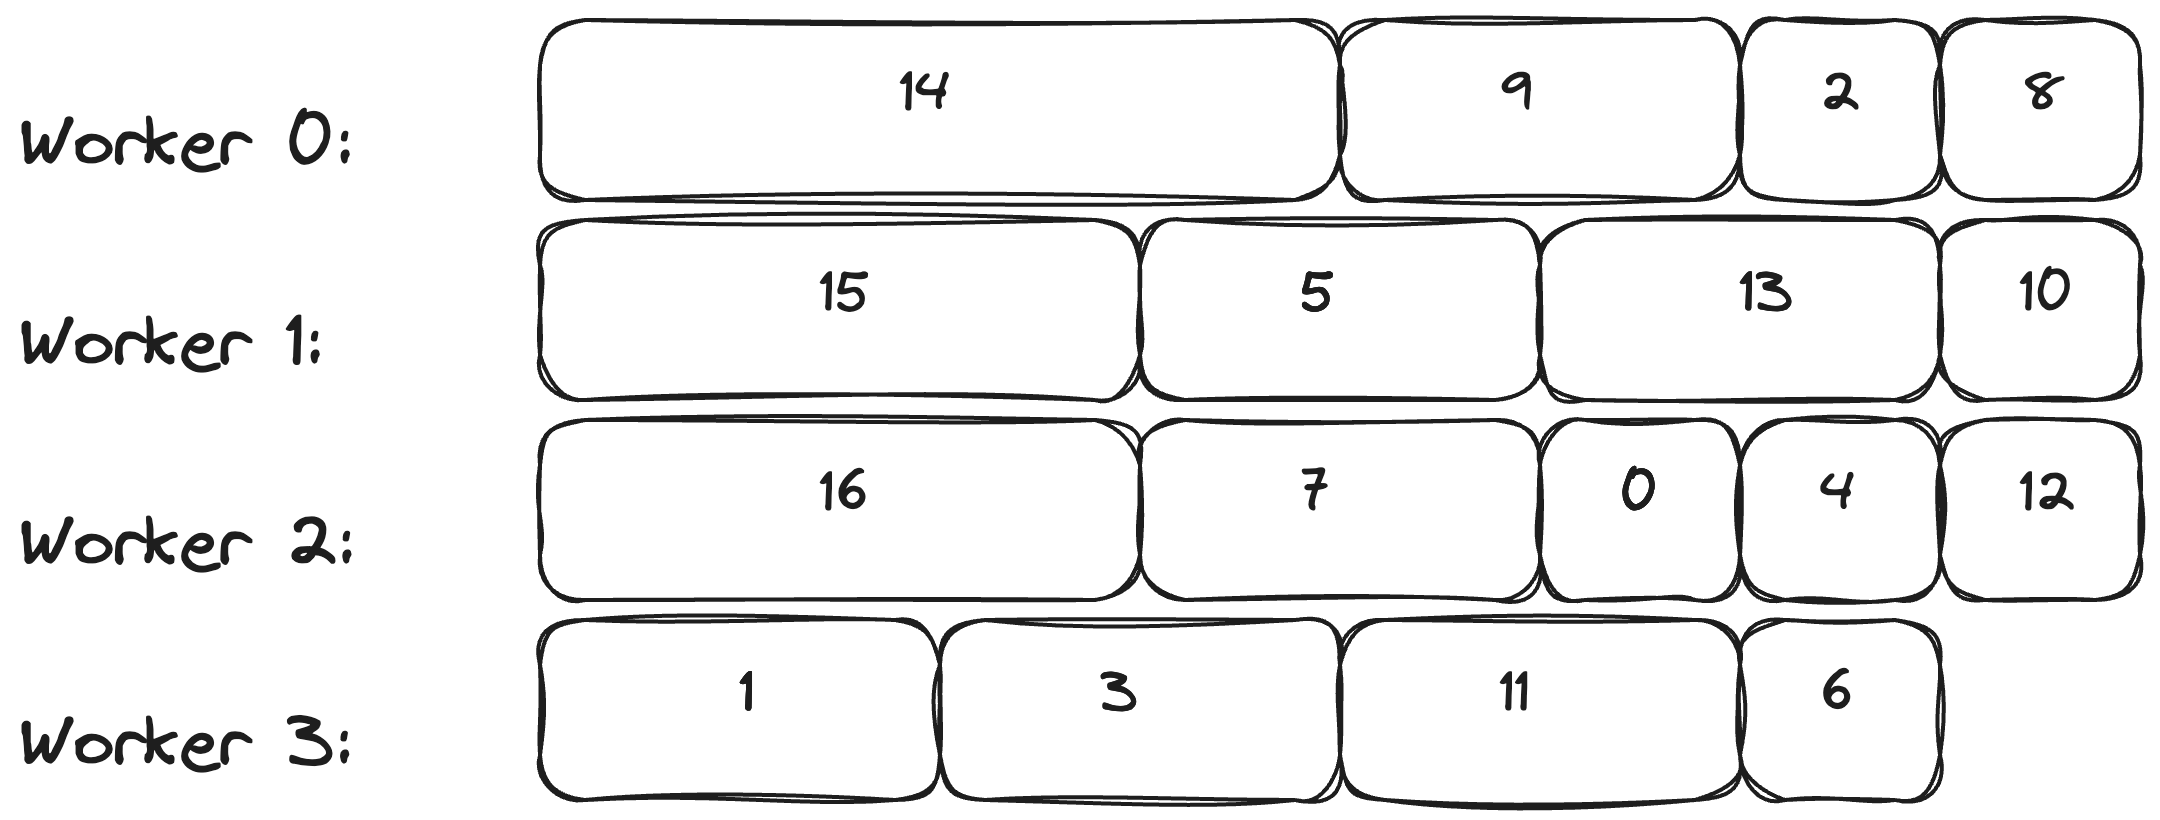
\includegraphics[width=0.75\textwidth]{./assets/gantt_lpt.png}
    \caption{Gantt chart of the LPT schedule (which happens to be optimal).}
    \label{fig:gantt_lpt}
\end{figure}

\subsection{Schedule \texttt{static,3}}

The schedule \texttt{static,3} assigns each task to a worker in a round-robin fashion with a chunk size of 3.

The makespan of the schedule \texttt{static,3} is 11, which is suboptimal compared to the LPT schedule. The Gantt chart in Figure \ref{fig:gantt_static3} shows the schedule.

\begin{figure}[htbp]
    \centering
    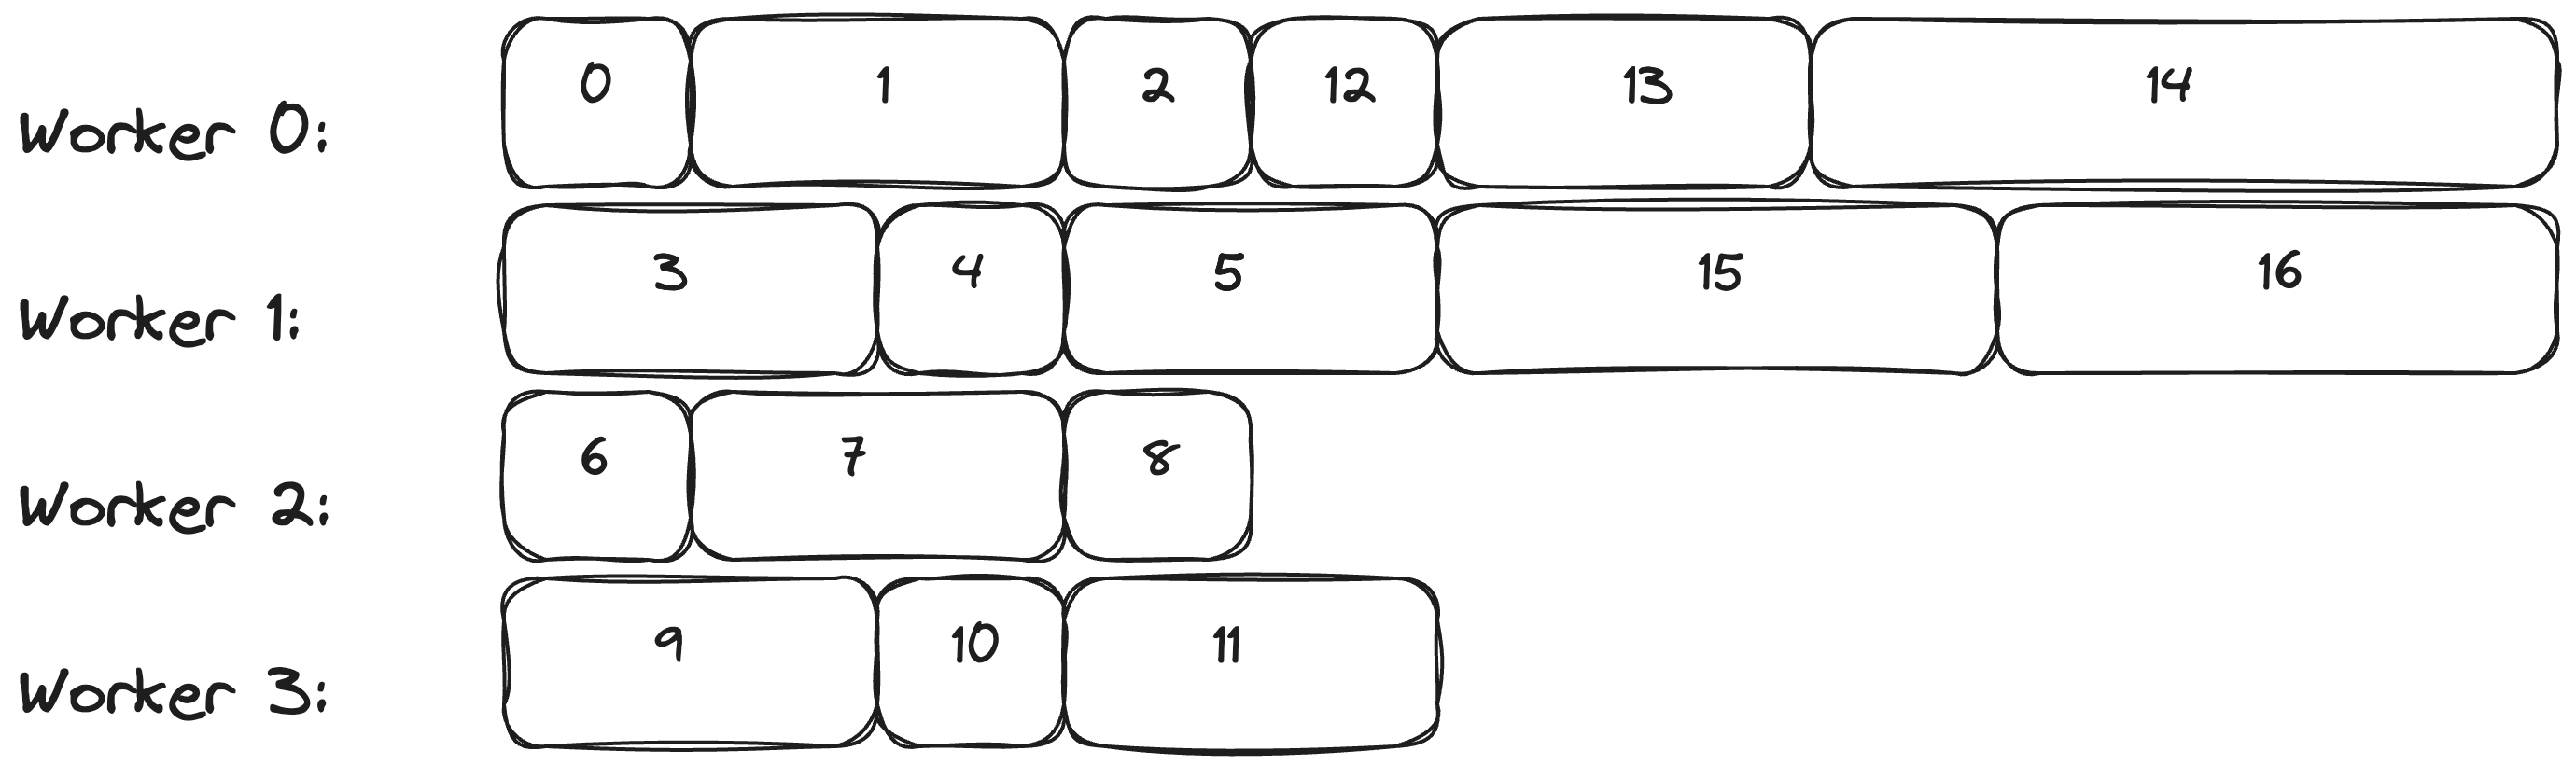
\includegraphics[width=0.75\textwidth]{./assets/static3.png}
    \caption{Gantt chart of the schedule \texttt{static,3}.}
    \label{fig:gantt_static3}
\end{figure}

\subsection{Schedule \texttt{dynamic,2}}

The schedule \texttt{dynamic,2} assigns chunks of 2 tasks to a random worker that is currently idle.

The makespan of the schedule \texttt{dynamic,2} is 10, which is suboptimal compared to the LPT schedule but better than the \texttt{static,3} schedule. The Gantt chart in Figure \ref{fig:gantt_static3} shows the schedule.

\begin{figure}[htbp]
    \centering
    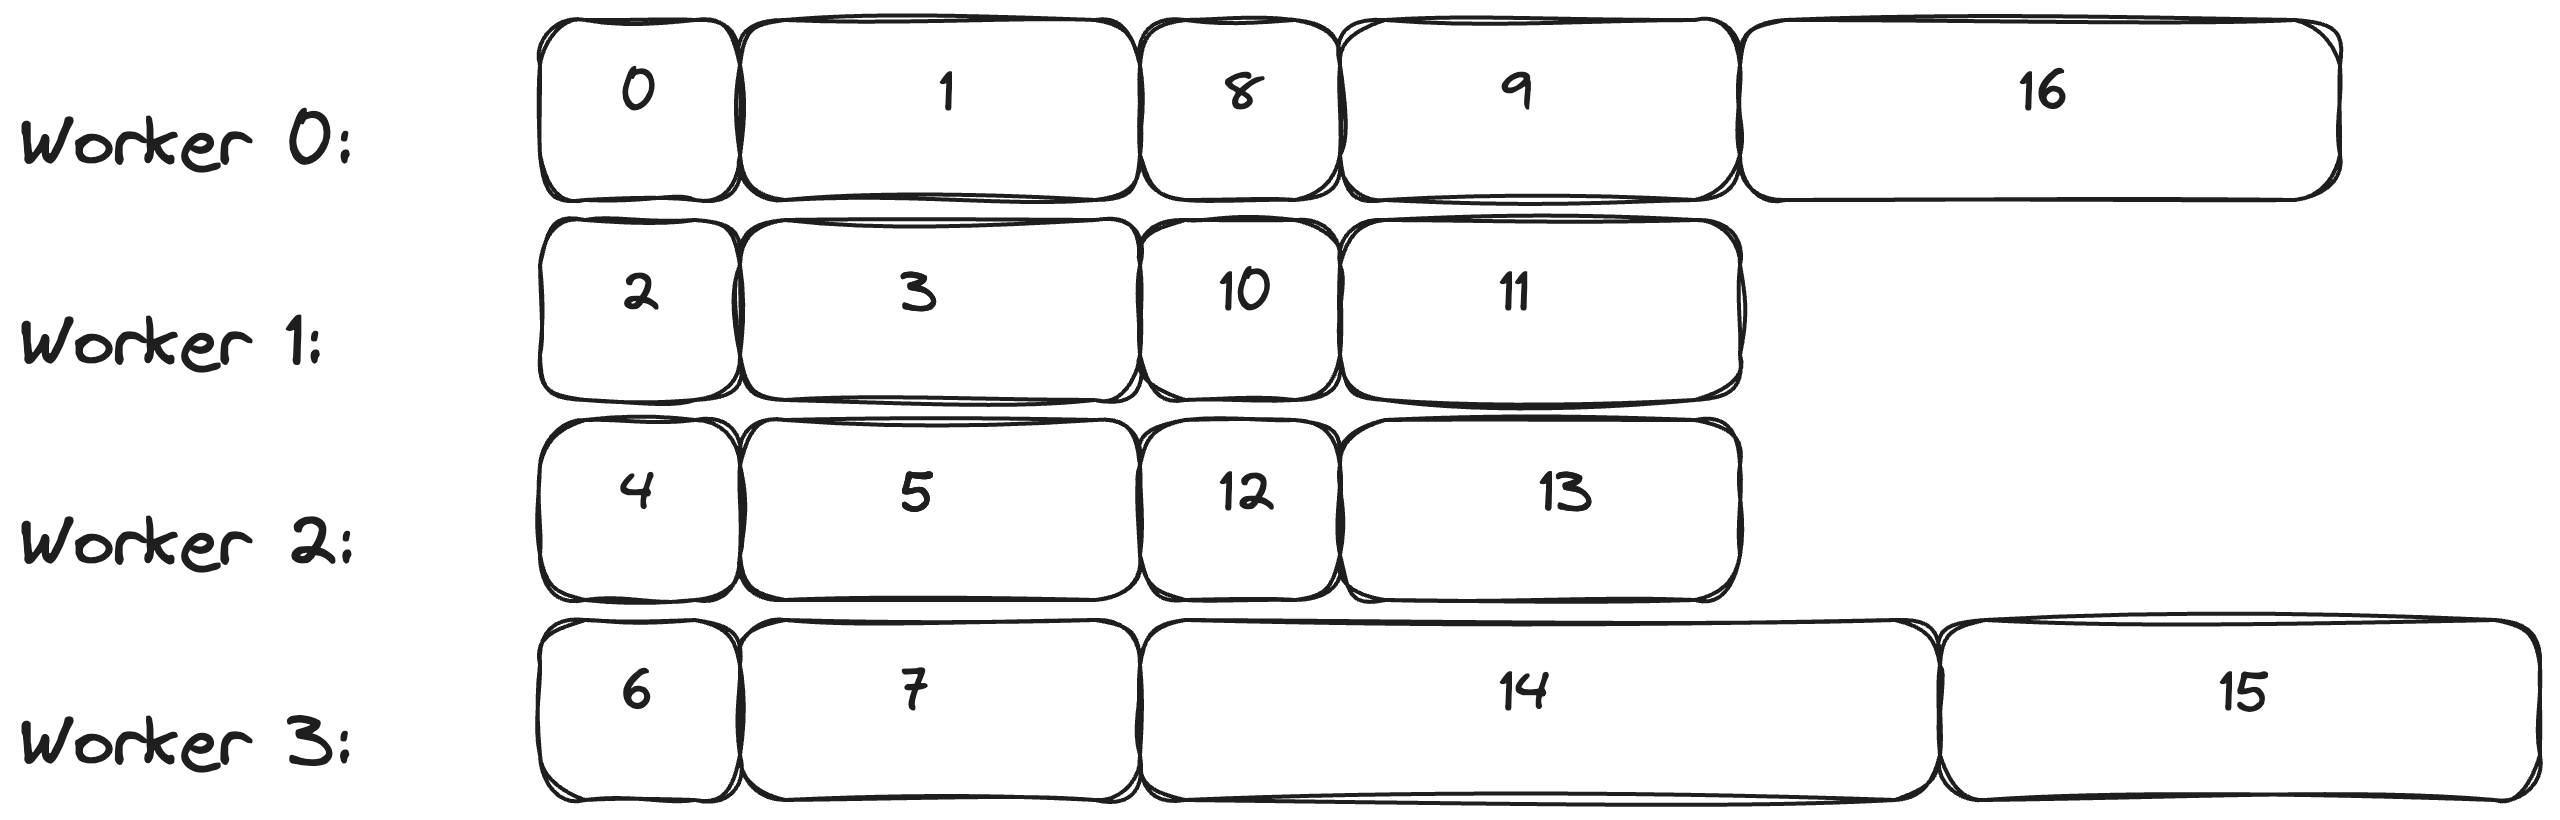
\includegraphics[width=0.75\textwidth]{./assets/dynamic2.png}
    \caption{Gantt chart of the schedule \texttt{dynamic,2}.}
    \label{fig:gantt_static3}
\end{figure}

\section{Exercise 3}

\subsection{Fix the problems with this OpenMP code}

Here are some suggestions to fix the problems with the given code snippet:

\begin{itemize}
    \item The instruction \texttt{count\_odd += my\_count\_odd;} doesn't make a lot of sense given that only the \texttt{\#pragma} region inside the \texttt{for} loop is parallelized. Replace the \texttt{my\_count\_odd} variable with the shared variable \texttt{count\_odd} and use an atomic operation to increment it. 

    \item Or even better: Use a reduction clause to sum up the number of odd numbers in the array instead of declaring a shared variable and incrementing it atomically yourself.
    
    \item Turn the function \texttt{static} so it's just visible in a single translation / compilation unit (optional).
\end{itemize}

\lstinputlisting{./demo/odd_counter.c}


\section{Exercise 4}

\subsection{What is the output of the three different versions?}

\subsection{How often is the function \texttt{omp\_tasks} called?}

\section{Exercise 5}

\subsection{Parallelize the pixel computation}

\subsection{Running time analysis}

\subsection{Influence of schedule parameter}

\section{Exercise 6}

\subsection{Parallelize the filter computation}

\subsection{Strong scaling analysis}

\subsection{Weak scaling analysis}

\newpage

\section{Addendum: Raw Data}

\begin{figure}[htbp]
    \centering
    \csvautotabular{./output/filter_strong.csv}\label{tab:filter_strong}
    \caption{Raw output from "filter strong" job.}
\end{figure}

\begin{figure}[htbp]
    \centering
    \csvautotabular{./output/filter_weak.csv}\label{tab:filter_weak}
    \caption{Raw output from "weak scaling" job. Timed out on \textit{slurmstepd} due to time out / time limit.}
\end{figure}

\begin{figure}[htbp]
    \centering
    \csvautotabular{./output/juliap.csv}\label{tab:juliap}
    \caption{Raw output from "juliap" job.}
\end{figure}

\begin{figure}[htbp]
    \centering
    \csvautotabular{./output/juliap2.csv}\label{tab:juliap2}
    \caption{Raw output from "juliap2" job.}
\end{figure}

\end{document}
